%%=====================================================================================
%%
%%       Filename:  data-structs-and-algs.tex
%%
%%    Description:  Formal notes of DS and A
%%
%%        Version:  1.0
%%        Created:  02/10/19
%%       Revision:  none
%%
%%         Author:  Josh Felmeden (), nk18044@bristol.ac.uk
%%   Organization:  
%%      Copyright:  Copyright (c) 2019, Josh Felmeden
%%
%%          Notes:  
%%
%%=====================================================================================

% Preamble {{{
\documentclass[11pt,a4paper,titlepage,dvipsnames,cmyk]{scrartcl}
\usepackage[english]{babel}
\typearea{12}
% }}}

% Set indentation and line skip for paragraph {{{
\setlength{\parindent}{0em}
\setlength{\parskip}{1em}
\usepackage[margin=2cm]{geometry}
\addtolength{\textheight}{-1in}
\setlength{\headsep}{.5in}
% }}}

\usepackage{hhline} 
\usepackage{mathtools} 
\usepackage[T1]{fontenc}

% Headers setup {{{
\usepackage{fancyhdr}
\pagestyle{fancy}
\lhead{Data Structures and Algorithms: The formal notes}
\rhead{Josh Felmeden}
\usepackage{hyperref} 
% }}}

% Listings {{{
\usepackage[]{listings,xcolor} 
\lstset
{
    breaklines=true,
    tabsize=3,
    showstringspaces=false
}

\definecolor{lstgrey}{rgb}{0.05,0.05,0.05}
\usepackage{listings}
\makeatletter
\lstset{language=[Visual]Basic,
    backgroundcolor=\color{lstgrey},
    frame=single,
    xleftmargin=0.7cm,
    frame=tlbr, framesep=0.2cm, framerule=0pt,
    basicstyle=\lst@ifdisplaystyle\color{white}\footnotesize\ttfamily\else\color{black}\footnotesize\ttfamily\fi,
    captionpos=b,
    tabsize=2,
    keywordstyle=\color{Magenta}\bfseries,
    identifierstyle=\color{Cyan},
    stringstyle=\color{Yellow},
    commentstyle=\color{Gray}\itshape
}
\makeatother
\renewcommand{\familydefault}{\sfdefault}
% }}}


% Other packages {{{
\usepackage{tikz-qtree}
\usepackage{tikz}
\usepackage{amssymb}
\usepackage{graphicx}
\graphicspath{ {./pics/} }
\usepackage{needspace}
\usepackage{tcolorbox}
\usepackage{soul}
\usepackage{babel,dejavu,helvet} 
\usepackage{amsmath} 
\usepackage{booktabs} 
\usepackage{tcolorbox} 
\usepackage[symbol]{footmisc} 
\renewcommand{\thefootnote}{\fnsymbol{footnote}}
\renewcommand{\familydefault}{\sfdefault}
% }}}

% tcolorbox {{{
\newtcolorbox{blue}[3][] {
    colframe = #2!25,
    colback = #2!10,
    #1,
}

\newtcolorbox{titlebox}[3][] {
    colframe = #2!25,
    colback = #2!10,
    coltitle = #2!20!black,
    title = {#3},
    fonttitle=\bfseries
    #1,
}
% }}}

% Title {{{
\title{Data Structures and Algorithms: The formal notes}
\author{Josh Felmeden}
% }}}

\begin{document}

\maketitle
\tableofcontents

\newpage
\section{Greedy algorithms}%
\label{sec:Greedy algorithms}
\subsection{Interval scheduling}%
\label{sub:interval-scheduling}
Let's suppose that you're running a satellite imaging service. Taking a
satellite picture of an area isn't instant and can take some time. It can
also only be done on the day where the satellite's orbit is lined up
correctly. Say you want to request some images to be taken from said
satellite, each of which can only be taken at certain times and you can
only take one picture at a time. How do we satisfy as many requests as
possible?

The requested satellite times that we have to deal with are: 12:00-12:30,
12:05-12:20, 12:15-12:55, 12:20-12:25, 12:38-12:50, and 12:45-13:00.

If we visualise this in a graph, we get: 


\begin{center}
    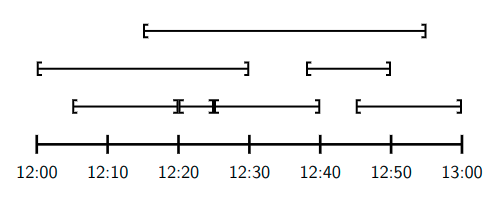
\includegraphics[scale=.5]{graph-satellite.png}
\end{center}

If we take a greedy algorithm approach to assigning these slots, we could
do something like assign the slot that finishes earliest, and then repeat
doing this until we have reached the end. For example, the slot that
finishes fastest is 12:05-12:20, so we assign this. This now removes the
ability for both 12:10-12:30 and 12:15-12:55 to be assigned, so we remove
these. This continues until we end up with something looking like this:


\begin{center}
    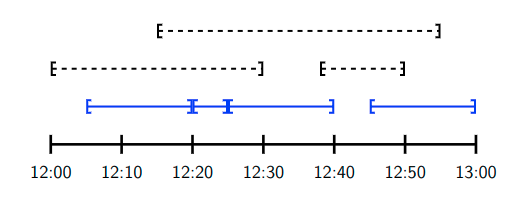
\includegraphics[scale=.5]{graph-assigned}
\end{center}

This means that we satisfy four requests (which is actually the maximum
possible, so well done us).

We can formalise this by saying that a \textbf{request} is a pair of
integers $(s,f)$ with $0 \le s \le f$.

\newpage
The algorithm that we're left with is this:
\begin{lstlisting}
public sub greedySchedule
    sort R
    for each i in {1 ... n} do
        if s_i >= lastf then
            A.append(s_i, f_i)
            lastf = f_i
        end if
    next
end sub
\end{lstlisting}

Now, we need to prove that the output is actually a \textbf{compatible
subset} of R. This is sort of intuitive because the set we added doesn't
break compatibility, since $s \ge$ \lstinline|lastf| and \lstinline|lastf|
is the latest finish time that's already in $A$.

We can formalise this with a loop invariant. At the start of the $i$th
iteration, we see that
\begin{itemize}
    \item $A$ contains a compatible subset $\{(S_1,F_1), \dots,
        (S_t,F_t)\}$ of R.
    \item \lstinline|lastf| = $\max(\{0\} \cup \{F_j : j \le t\})$ 
\end{itemize}

The base case ($i=0$) is immediate because $A = []$. The induction step is
that $A$ was compatible at the start of the iteration, and therefore if we
append a pair $s_i,f_i$ to $A$ then $s \ge $ \lstinline|lastf| $\ge F_j$
for all $f \le t$. This means that $(s_i,f_i)$ is compatible with $A$.


\begin{titlebox}{blue}{Greedy algorithms definition}
Greedy algorithms are actually an informal term and people have different
definitions. The definition that we're going to use is:
\begin{itemize}
    \item They start with a sub-optimal solution.
    \item They look over all the possible improvements and pick the one
        that looks the best at the time.
    \item They never backtrack in `quality'.
\end{itemize}
\end{titlebox}

Greedy algorithms might fail; it's not enough to just do the obvious thing
at each stage. While the algorithms might fail initially, we can use the
knowledge that we gained from the results of the algorithm to design a
more correct one.

\section{Graphs}%
\label{sec:Graphs}

\begin{titlebox}{blue}{Graph Definition}
        A \textbf{graph} is a pair $G = (V,E)$ where $V=V(G)$ is a set of
        \textbf{vertices} $E = E(G)$ is a set of \textbf{edges} contained
        in $\{\{u,v\} : u,v \in V, u \not = \}$
\end{titlebox}

\begin{titlebox}{blue}{Walk Definition}
        A \textbf{walk} in a graph $G = (V, E)$ is a sequence of vertices
        such that $\{v_i, v_{i+1} \in E \text{ for all } i\le k-1$

        We say that the walk is from $v_0$ to $v_k$ and call $k$ the
        length of the walk.
\end{titlebox}


\subsection{Euler walks}%
\label{sub:Euler walks}
An \textbf{Euler walk} is one that contains every edge in $G$
exactly once.

Two graphs might be \textbf{equal}. This is the case when two graphs $G_1
= (V_1, E_1)$ and $G_2 = (V_2, E_2)$ are equal and written $G_1 = G_2$ if
$V_1 = V_2$ and $E_1 = E_2$. This does present some issues, however,
because sometimes graphs look like they should be equal, when they're not
because the edges are labelled differently.

This is where \textbf{isomorphism} comes in. $G_1$ and $G_2$ are
\textbf{isomorphic} if there's a bijection $f: V_1 \rightarrow V_2$ such
that $\{f(u),f(v) \} \in E_2$ if and only if $\{u,v\} \in E_1$.

Intuitively, this means that $G_1 \xrightarrow{\sim} G_2$ if they are the
same graph but the vertices are relabelled.

In a graph $G = (V,E)$, the \textbf{neighbourhood} of a vertex $v$ is the
set of vertices joined to $v$ by an edge. Formally, 
$N_G(v) = \{w \in V : \{v,w\} \in E$. Also, for all sets of vertices
$X \subseteq V = \cup_{v\in X} N_G(v)$

The \textbf{degree} of a vertex $v$ is the \textbf{number} of vertices
joined to $v$. Formally: $d_G(v) = |N_G(v)|$

\textbf{Theorem}: If $G$ has an Euler walk, then either:
\begin{itemize}
    \item Every vertex of $G$ has even degree or
    \item All but two vertices $v_0$ and $v_k$ have even degree, and any
        Euler walk must have $v_0$ and $v_k$ as endpoints.
\end{itemize}

Does every single graph that satisfies both of these conditions have an
Euler walk? No, because the graphs need to be \textbf{connected}.

Within a graph, we also have subgraphs and induced subgraphs. A
\textbf{subgraph} $H = (V_H, E_H)$ of $G$ is a graph with $V_H \subseteq$
and $E_H \subseteq E$. $H$ is an \textbf{induced subgraph} if $V_H
\subseteq V$ and $E_H = \{ e \in E : e \subseteq V_H\}$.

For all vertex sets $X \subseteq V$, the graph is \textbf{induced} by $X$
is:

\begin{center}
    \begin{align*}
        G[X] = (X, \{e \in E: e \subseteq X \})
    \end{align*}
\end{center}

A \textbf{component} $H$ of $G$ is the maximal connected induced subgraph
of $G$, so $H = G[V_H]$ is connected, but $G[V_H \cup \{v\}]$ is
disconnected for all $v \in V \backslash V_H$.

\begin{blue}{blue}
    \textbf{Theorem}: Let $G = (V,E)$ be a \textbf{connected} graph, and
    let $u,v \in V$. Then, $G$ has an Euler walk from $u$ to $v$ if and
    only if either:
    \begin{enumerate}
        \item $u = v$ and every vertex of $G$ has even degree, or
        \item $u \not = v$ and every vertex of $G$ has even degree except
            $u$ and $v$.
    \end{enumerate}
\end{blue}

\section{Sequential Processes}%
\label{sec:sequential-processes}

\section{Fast Fourier Transform}%
\label{sec:fft}

\subsection{Polynomials}%
\label{sub:Polynomials}
A \textbf{degree} $n-1$ polynomial in $x$ can be seen as a function:

\begin{align*}
    A(x) = \sum^{n-1}_{i=0}a_i \cdot x^i
\end{align*}

Any integer that's bigger than the degree of a polynomial is a
\textit{degree bound} of said polynomial. The polynomial $A$ is:

\begin{align*}
    a_0 \cdot x^0 + a_1 \cdot x^1 + a_2 \cdot x^2 \cdots + a_{n-1}x^{n-1}
\end{align*}

The values $a_i$ are the \textit{coefficients}, the degree is $n-1$ and
$n$ is a degree bound. We're able to express any integer as some kind of
polynomial by setting $x$ to some base, say for decimal numbers:

\begin{align*}
    A = \sum^{n-1}_{i=0} a_i \cdot 10^i
\end{align*}

The variable $x$ just allows us to evaluate the polynomial at a point. A
really fast way to evaluate the polynomial is to use \textbf{Horner's
Rule}.

\begin{titlebox}{blue}{Horner's Rule}
Instead of computing all the terms individually, we do:
\begin{align*}
    A(3) = a_0 + 3 \cdot (a_1 + 3\cdot (a_2 + \cdots + 3\cdot (a_{n-1})))
\end{align*}

This method requires $O(n)$ operations. For example, if we consider $A(x) = 2 + 3x + 1.x^2$, we can evaluate this
as:
\begin{align*}
    A(x) = 2 + x(3 + 1.x)
\end{align*}

\end{titlebox}

Once we have our polynomial representations, we might be doing some
arithmetic with them. We're allowed to write polynomials in a
\textit{coefficient representation}. Here, the addition of $C = A + B$
constructs $C$ as the vector:

\begin{align*}
    (a_0 + b_0, a_1 + b_1, a_2 + b_2, \dots, a_{n-1} + b_{n-1})
\end{align*}

$A$ and $B$ should really have the same length, but we're allowed to just
pad the coefficients with zero to make this the case.

\subsubsection{Point value Representation}%
\label{ssub:point-value}
We know that if we're given a polynomial, we can graph it. We can use this
fact to represent a polynomial as a list of its points. For point value
representation, the addition $C = A + B$ constructs $C$ as:

\begin{align*}
    \{x_0, y_0 + z_0),(x_1,y_1 + z_1),(x_2,y_2 + z_2), \dots,
        (x_{n-1},y_{n-1} + z_{n-1})
\end{align*}

where $x_i$ is a point, $y_i = A(x_i) and z_i = B(x_i)$.

It's important to note that the two value representations \textbf{must}
use the same evaluation points. Both of the operations are $O(n)$ in
terms of how long they take.

\subsubsection{Polynomial multiplication}%
\label{ssub:convolution}
Computing a polynomial multiplication (also called \textbf{convolution})
is a little harder than addition. It does, however, become much easier
when we use point value representation:

\begin{align*}
    \{x_0, y_0 \cdot z_0),(x_1,y_1 \cdot z_1),(x_2,y_2 \cdot z_2), \dots,
        (x_{n-1},y_{n-1} \cdot z_{n-1})
\end{align*}

where $x_i$ is a point, $y_i = A(x_i) and z_i = B(x_i)$.

The normal method of calculating multiplication is $O(n^2)$, while using
point value representation only takes $O(n)$. So, is there an easy way to
convert to point value representation? Actually, yes. What we need to do
is to evaluate the polynomial to a point-value representation, multiply
and finally interpolate (the opposite of evaluating) back again.

Long story short, we need to develop two fast algorithms that construct
the coefficients for the point value representation and then
interpolate. So the main steps to multiply the two polynomials $A$ and $B$
(of degree $n$) are:

\begin{enumerate}
    \item \textit{Double degree bound}: Create coefficient representations
        of $A(x)$ and $B(x)$ as degree bound $2n$ polynomials by adding
        $n$ high-order zero coefficients to each.
    \item \textit{Evaluate}: Compute point-value representations of $A(x)$
        and $B(x)$ of length $2n$ through two applications of FFT of order
        $2n$
    \item \textit{Pointwise multiply}: compute a point-value
        representation of $cC(x) = A(x)B(x)$ by multiplying the values
        Pointwise
    \item \textit{Interpolate}: Create a coefficient representation of
        $C(x)$ through a single application of the \textit{inverse} FFT.
\end{enumerate}

The first and third steps are really easy to perform in $O(n)$ time. The
claim is that if we evaluate at the complex roots of unity then we can
perform steps 2 and 4 in $O(n \log n)$ time.

\subsection{Evaluation at roots of unity}%
\label{sub:roots-unity}
First, we need to look at evaluation. We need to evaluate a polynomial of
degree $n$ at $n$ different points. It appears that the complexity of our
method is just going to be $O(n^2)$, but there is a faster way of doing it
than just using Horner's rule. This is when we evaluate the points at
\textit{special} points (namely the \textbf{N-th complex roots of unity}).

\begin{titlebox}{blue}{N-th complex roots of unity}
    \begin{itemize}
        \item The roots of unity are the values $\omega_N = e^{2\pi i j /
            N}$ for $j = 0,1,\dots,N-1$
        \item Say we are evaluating at $N$ pints, we take the N-th complex
            roots of unity $\omega_N$
        \item This means we evaluate the polynomial at the points:
            \begin{align*}
                \omega_N^0,\omega_N^1,\omega_N^2,\dots,\omega_N^{n-1}
            \end{align*}
    \end{itemize}
\end{titlebox}

We want to evaluate a polynomial A at the $n$ roots of unity. Therefore,
we evaluate:
\begin{align*}
    A(x) = \sum_{j=0}^{n-1}a_j \omega_n^{kj}
\end{align*}

for every $k = 0,1,\dots, n-1$

We define the vector of results of these evaluations as:

\begin{align*}
    y_k = A(\omega^k_n)
\end{align*}

This vector $y = (y_0, \dots, y_{n-1})$ is the \textbf{discrete Fourier
Transform} (DFT) of the coefficient vector $a = (a_0, a_1, \dots, a_{n-1})$

\begin{titlebox}{blue}{The Cancellation Lemma}
\begin{align*}
    \omega^{dk}_{dN} = \omega^{k}_{N}
\end{align*}
\end{titlebox}

\begin{titlebox}{blue}{The Halving Lemma}
    If $N > 0$ is even then the squares of the $N$ complex N-th roots of
    unity are the $N/2$ complex $N/2$-th roots of unity

    The proof of this is that we have $(\omega^k_n) ^2 = \omega^k_{n/2}$
    for any nonnegative integer $k$ because of the cancellation lemma.
\end{titlebox}

\subsection{Fast Fourier Transform}%
\label{sub:fft}
The really basic idea of the Fast Fourier transform is that we define two
new polynomials;

\begin{align*}
    A^{[0]}(x) = a_0 + a_2x + \cdots + a_{N-2}x^{N/2 - 1} \\
    A^{[1]}(x) = a_1 + a_3x + \cdots + a_{N-1}x^{N/2 - 1}
\end{align*}

%08/11/19
\section{Dynamic Programming}%
\label{sec:dynamic-programming}
We use \textit{dynamic programming} for finding efficient algorithms for
problems that can be broken down into simpler, overlapping subproblems.
Basically,
\begin{enumerate}
    \item Find a recursive formula for the problem (in terms of answers to
        the subproblems)
    \item Write down a naive recursive algorithm
    \item Speed it up by storing the solutions to the subproblems (\textbf{memoization})
    \item Derive an iterative algorithm by solving the subproblems in good
        order.
\end{enumerate}

\subsection{Weighted interval scheduling}%
\label{sub:weighted-scheduling}
We've seen the scheduling problem before on the course, but this is
different (and as it turns out, harder).

A \textbf{schedule} is a set of compatible intervals. The \textit{weight}
of a schedule is the sum of the weight of the intervals it contains.

We could use a greedy algorithm, but it is really slow and not what we're
looking for. It's not even going to cut it full stop.

\subsubsection*{How is the input provided?}
The intervals are given in an array $A$ of length $n$.

$A[i]$ stores a triple $(s_i, f_i, w_i)$ which defines the $i$th interval.

The intervals are sorted by finish time i.e. $f_i \le f_{i+1}$.=, or the
interval $i$ finishes before the interval $i+1$ finishes.

\subsubsection*{Compatible Intervals}
For all $i$, we let $p(i)$ to be the rightmost interval (in order of
finish time) which finishes before the $i$th interval but doesn't overlap
it.

In the below example, if we take $i = 7$, $p(7) = 3$ because it's the
first interval that doesn't overlap with it (and 3 is the position of the
interval in the array).

\begin{center}
    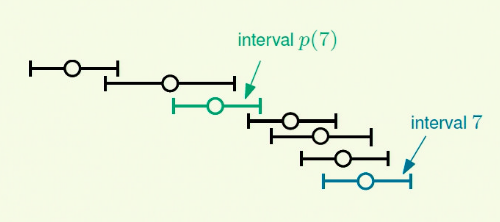
\includegraphics[scale=.5]{weighted-int.png}
\end{center}

$p(4) = 2$, and $p(2) = 0$ because there is no interval that exists.
\textbf{Note} that we index from 1 because otherwise 0 would not make
sense.

\textbf{Claim.} We can precompute all $p(i)$ in $O(n \log n)$ time. For
now, we can assume that this is true, but I will revisit this and prove
why. If you did it naively, it would be $O(n^2)$ time. Obviously it's
something to do with dynamic programming (because that's what this section
is about).

\subsubsection{Finding a solution}%
\label{ssub:solution-dynamic}
Consider some optimal schedule $\mathcal{O}$ for intervals $\{1, 2, 3,
\dots, n\}$ with weight $OPT$. Now, either the $n$th interval is in
schedule $\mathcal{O}$ or it isn't.

Let's look at the case where it is not in $\mathcal{O}$. Schedule
$\mathcal{O}$ is also an optimal schedule for the problem with the input
consisting of the intervals $\{1, 2, 3, \dots, n-1\}$ because $n$ is not in
it. Therefore, in this case, we have $OPT = OPT(n-1)$. (By the way,
$OPT(i)$ is the weight of an optimal schedule for the intervals $\{1,
2, 3, \dots, i\}$).

Now, let's consider the case that it \textbf{is} in $\mathcal{O}$. The
only other intervals that could be in $\mathcal{O}$ are $\{1, \dots,
p(n)\}$. We know that everything larger than $p(n)$ is incompatible with
the $n$th schedule.

\begin{center}
    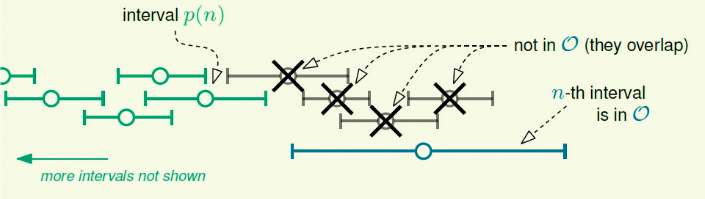
\includegraphics[scale=.5]{weight-n-sched.png}
\end{center}

Schedule $\mathcal{O}$ with interval $n$ removed gives an optimal schedule
for the intervals $\{1, 2, \dots, p(n) \}$ so we now have that $OPT =
OPT(p(n)) + w_n$.

To summarise:
\begin{itemize}
    \item \textbf{Case 1}: The $n$th interval is not in $\mathcal{O}$,
        then $OPT = OPT(n-1)$
    \item \textbf{Case 2}: The $n$th interval is in $\mathcal{O}$, then
        $OPT = OPT(p(n)) + w_n$
\end{itemize}

So, which one do we choose? We choose the bigger one:

\begin{align*}
    OPT = \max (OPT(n-1),OPT(p(n)) + w_n)
\end{align*}

We just now replace all $n$ with $i$ to give us our final recursive
algorithm

\begin{align*}
    OPT = \max (OPT(i-1),OPT(p(i)) + w_i)
\end{align*}

There's no easy way to find these solutions, you just have to kind of look
at the problem for a while and then it will come to you.

\subsubsection{Writing down the recursive algorithm}%
\label{ssub:recursive-written}
Now we have the formula, we get the recursive algorithm:

\begin{lstlisting}
WIS(i)
    If (i=0)
        Return 0
    Return max(WIS(i-1),WIS(p(i)) + wi)
\end{lstlisting}

This algorithm is pretty much exponential given the wrong input. If $T(n)$
is the run time of WIS($n$) using overlapping intervals, then $T(n) >
2T(n-1)$. This is $O(2^{n/2})$.

\subsubsection{Memoization}%
\label{ssub:Memoization}
To solve this, we need to store the solutions to the subproblems.

\begin{lstlisting}
MEMWIS(i)
    If (i=0)
        Return 0
    If WIS[i] undefined
        WIS[i] = max(MEMWIS(i-1),MEMWIS(p(i)) + wi)
    Return WIS[i]
\end{lstlisting}

In this algorithm, we store the solutions to the previously computed
subproblems in an $n$ length array called WIS. The time complexity of
computing MEMWIS($n$) is now $O(n)$. Unfortunately, linear recursion is
still kind of bad.

To compute a value in the array WIS[$i$], we need both WIS[$i-1$] and
WIS[$p[i]$]. Both of these are to the left of WIS[$i$]. Therefore, we
should go through this array from left to right. This is because every
time we compute something, we already have all of the things we need. This
gives us a new algorithm:

\begin{lstlisting}
ITWIS(n)
    If (i=0)
        Return 0
    For i=1 to n
        WIS[i] = max(WIS[i-1], WIS[p(i)] + wi)
\end{lstlisting}

This is an iterative dynamic programming algorithm that runs in $O(n)$
time. The iterative method is better because if we use recursion in $O(n)$
time, we'll probably overload the stack, so this makes the memory
footprint of the algorithm now much smaller. It \textbf{does} however mean
that we need to precompute the $p(i)$ values.

\subsubsection{Computing the p(i) function}%
\label{ssub:Computing the p(i) function}
\textbf{Revised claim.} We can precompute any $p(i)$ in $O(\log n)$ time.
Remember that $s_i$ is the start of interval $i$ and $f_i$ is the finish
time of interval $i$. We want to find the unique value $j = p(i)$ such
that:

\begin{align*}
    f_j < s_i < f_{j+1}
\end{align*}

Because the input is sorted by finish times, we can find $j$ just by using
binary search in $O(\log n)$ time. We can now precompute all $p(i)$ in
$O(\log n)$ time.

% 11/11/19
\section{Dynamic search structures}%
\label{sec:dynamic-search}
A dynamic search structure stores a set of elements. Each element $x$ must
have a unique key: \lstinline|x.key|. The following operations are
supported:

\begin{itemize}
    \item \lstinline|insert(x,k)|: inserts \lstinline|x|  with key \lstinline|k = x.key| 
\end{itemize}
% TODO this

\subsection{Binary search trees}%
\label{sub:bin-search-tree}
Remember that in a binary search tree:
\begin{itemize}
    \item All the nodes in the left subtree have smaller keys
    \item All the nodes in the right subtree have larger keys
\end{itemize}

We perform a \lstinline|find| operation by following a path from the root.

%\begin{tikzpicture}
%    \Tree
%    [.27
%    [.21]]
%\end{tikzpicture}
%% TODO draw a tree

\subsection{2-3-4 Trees}%
\label{sub:2-3-4 Trees}
The idea of this tree is that the nodes can have anywhere between 2 and 4
children (\textit{hence the name}).

\textbf{Perfect balance} means that every path from the root to a leaf has
the same length. Always. Forever.

\begin{itemize}
    \item \textbf{2-node}: 2 children and 1 key
    \item \textbf{3-node}: 3 children and 2 keys
    \item \textbf{4-node}: 4 children and 3 keys
\end{itemize}

Like in a binary search tree, the keys held at a node determine the
contents of its subtrees.

Just like in a binary tree, we have a \lstinline|find| operation. We
perform the operation by following a path from the root. Decisions are
made by inspecting the keys at the current node and following the
appropriate edge.

The time complexity of the \lstinline|find| operation is $O(h)$ again.

\subsubsection{The insert operation}%
\label{ssub:insert}
To perform \lstinline|insert(x,k)|, we need to:
\begin{enumerate}
    \item Search for the key \lstinline|k|  as if we were performing
        \lstinline|find(k)|.
    \item If the leaf is a 2-node, then we insert \lstinline|(x,k)| and
        convert it into a 3-node.
    \item If the leaf is a 3-node, then we insert \lstinline|(x,k)| and
        convert it into a 4-node.
    \item If the leaf is a 4-node, we just make sure it never happens.
\end{enumerate}

\subsubsection{Splitting 4-nodes}%
\label{ssub:split-4-nodes}
We can \lstinline|split| any 4-node into two 2-nodes \textit{if} its
parent isn't a 4-node. For example:

%TODO draw this operation (tikzpicture) Also learn how to use tikz picture
%it seems really useful

We push the extra key up to the parent (which wouldn't work if the parent
is a 4-node). The subtrees haven't changed size, so the path lengths have
not changed due to this \lstinline|split| operation. Therefore, if it was
\textbf{perfectly balanced} before, then it's perfectly balanced after.

\lstinline|splitting| the root increases the height of the tree and
increases the length of all the root-leaf paths by one so it maintains the
\textbf{perfect balance} property. This is the only way that
\lstinline|insert| can affect the lengths of the paths.

Each \lstinline|split| takes $O(1)$ time, so overall \lstinline|insert|
takes $O(\log n)$ time.

\subsubsection{Other operations}%
\label{ssub:other-ops}

\lstinline|Fuse| is an operation that combines two 2-nodes (with the same
parent) into a 4-node (provided the parent isn't a 2-node).

\lstinline|Transferring| keys is possible. If there is a 2-node and a
3-node, we can perform a \lstinline|Transfer| (even if the parent is the
root). No path lengths change from this operation and the time taken is
$O(1)$ time.

\subsubsection{Deleting a node}%
\label{ssub:delete}
To perform \lstinline|Delete(k)| on a \textbf{leaf}, we:
\begin{enumerate}
    \item Search for the key \lstinline|k| using \lstinline|find(k)|. We
        use \lstinline|fuse| and \lstinline|transfer| to convert the
        2-nodes as we go down.
    \item If the leaf is a 3-node, we delete \lstinline|(x,k)|
        %TODO finish this
\end{enumerate}

If we \lstinline|fuse| the root, then the height can decrease by 1. This
is the only time the tree can decrease in height.

If we want to \lstinline|delete| something other than a leaf, we need to:
\begin{enumerate}
    \item Find the \textbf{predecessor} of \lstinline|k| (this is the same
        as \lstinline|find|). This is the element with the largest key
        $k'$ such that $k' < k$
    \item Call \lstinline|delete(k')|. Fortunately, \lstinline|k'| is
        always a leaf
    \item Overwrite \lstinline|k| with another copy of \lstinline|k'|.
\end{enumerate}

\subsection{Summary}%
\label{sub:Summary}
A 2-3-4 tree is a data tructure that's based on a tree structure. they are
a little awkward to implement because all nodes don't have the same number
of children. So in practice, we use something called a
\textbf{red-black} tree. It is similar to a binary tree and supports
\lstinline|insert|, \lstinline|find|, \lstinline|delete| functions.

Why do we bother learning these 2-3-4 trees then? Well, they're a little
bit nicer and less complicated to think about and they're basically the
same structure.

%12/11/19
\section{Making shortcuts}%
\label{sec:shortcuts}
What happesn if we add some shortcuts to a set of nodes. Because in the
real world it's possible to take shortcuts in terms of a train line or
something similar.

We might attach a second linked list containing only some of the keys. How
do we now perform \lstinline|find(k)| in this linked list?

To perform \lstinline|find| we start in the top list and go right until
we.  come ot a key $k' > k$. Then, we move down to the bottom list and go
right until we find $k$. Imagine that we decide to place $m$ keys in the
top list, and the bottom list contains $n$ keys (this will always be true
since the bottom list has all of the keys). Where should we put the $m$
keys to minimise the the \textit{worst} case (for a find operation)?

If we spread out the $m$ keys evenlt, we get the biggest overall
improvement. If we do an uneven spread, some of the keys will be found
really fast, but there will be some poor cases, and since we're trying to
minimise the worst case, we want to make sure all cases are catered for.
Now, the worst case time for a \lstinline|find| operation becomes $O(m +
n/m)$.

By setting $m = \sqrt{n}$, we get the \textbf{worst case} time for a
\lstinline|find|  operation to be $O(\sqrt{n})$.

\subsection{More levels}%
\label{sub:levels}
We've looked at having 2 lists, but what if we have more than that? The
more levels we interoduce, the better it gets. Each \textit{level} will
contain \textbf{half} of the keys (called rounding up) from the level
below. They are chosen to be spread as evenlt as possible.

The bottom level still contains every key, and every level contains the
leftmost and rightmost keys.

since each level has half of the keys from hte below level, there are
$O(\log n)$ levels (kinda like a tree). 

% Write hte notes from this lecture my laptop died TODO

% lecture from 15/11/19
\section{Line segments}%
\label{sec:line-segments}
Consider $n$ line segments. Find all of the intersections. How do we go
about this?

The simplest algorithm is to test every pair of line segments.

Let $s_i$ denote the $i$-th line intersection:
\begin{lstlisting}
for i = 1,2, ..., n
    for j = 1,2, ...,n
        if (s[i] intersects s[j]) and (i != j)
            output (i,j)
\end{lstlisting}

Given two line segments $s_i$ and $s_j$, described by their end point
coordinates, we can decide whether (and also where) they intersect in
$O(1)$ time. This can be proved because any computation on two objects
with $O(1)$ (constant) space descriptions take $O(1)$ time. It doesn't
tell you how to do it, but just know that this is true.

The algorithm above, however, runs in $O(n^2)$ time (because checking each
pair of lines takes $O(1)$ time).

If there are $n$ line segments we could have a maximum of $(n/2)^2$
intersections. If we want to output all of the intersections, then we
can't expect to do better than $O(n^2)$ in the worst case simply because
the time complexity of printing the output.

\subsection{Output sensitive algorithms}%
\label{sub:ouput-sensitive}
Up to this point in the course, we've only looked at how the actual
input affects the runtime. With this algorithm, however, we also need
to consider the size of the output.

Eventually, we'll work up to an algorithm with runtime $O(n \log n + k
\log n)$. When $K$ is really big, then this algorithm is actually worse
than the naive algorithm with $O(n^2 \log n)$. But, when $k$ is small, the
algorithm is much better with $O(n \log n)$.  

\newpage
\subsection{Simplifying restrictions}%
\label{sub:simplifying-restriction}
To make things a bit easier, we are not allowing:
\begin{itemize}
    \item Horizontal line segments
    \item Two end points with the same %y% coordinates
    \item Three or more line segments that intersect at the same point
    \item Overlapping line segments
\end{itemize}

\subsection{First observation}%
\label{sub:first-ob}
The \textbf{$y$-span} of $s_i$ is the range of the $y$ axis that $s_i$
takes. From this definition, if $s_i$ and $s_j$ don't have overlapping
$y$-spans, they don't intersect. This method suggests an overall approach
called \textit{line sweeping}. We sweep a horizontal line through the
plane from top to bottom and find intersections as we go.

When we see that there are two lines in the same $y$-span that are also
next to each other, we say that the two lines are \textit{adjacent}
\textbf{at this $y$-coordinate}. Some pair of lines that are adjacent at
some $y$ coordinate may not be adjacent at another because another line
might come between them.

\textbf{Note!} Two line segments that are \textit{never} adjacent
\textbf{cannot intersect}. Intuitively, if they are never actually next to
each other, they cannot cross.

\subsubsection{Event points}%
\label{ssub:event-points}
The \textbf{event points} are the `interesting positions' of a line, which
we define as the end points of the line and the intersection points. We
have to detect the intersection points on the fly \textbf{before} we get
to them.

The total number of event points is $O(n + k)$ where $n$ is the number of
endpoints and $k$ is the number of intersections.

\subsubsection{Status of the sweep line}%
\label{ssub:status-sweep-line}
The status of the sweep line is the set of line segments that currently
intersect the sweep line. We order this from \textit{left to right} by
where they intersect.

The status of the sweep line can only change at event points.

We will store the status of the sweep line in a data structure. This allows
efficient updates.

\subsubsection{Updating the sweep line}%
\label{ssub:update-sweep-line}
Every time the sweep line moves to the next event point, we update the
status data structure. If the event point is the \textit{top of a line
segment}, we insert it into the status data structure at the appropriate
place (using the insert function).

Then, we check whether the segment will intersect either of the adjacent
segments.

If the event point is the \textit{bottom of a line segment} then we delete
it from the status data structure.

Finally, if the event point is an \textit{intersection point}, we
\textbf{swap} the two line segments in the data structure.

% Lecture from 25/11/19
\section{Shortest Path Revisited}%
\label{sec:shortest-path-revisited}
We've already looked at the shortest path thing, but now, we're going to
do it with negative weights. Bellman-Ford's algorithm solves the
\textbf{single source shortest paths} problem (in a weighted directed
graph).

It finds the shortest path from a given \textit{source} vertex to every
other vertex. The weights are allowed to be both positive and negative,
and the graph is stored as an \textbf{adjacency list}.

\subsection{Negative weight cycles}%
\label{sub:negative-cycles}
If some of the edges in the graph have negative weights, the idea of a
shortest path might not make sense:

%TODO draw a negative cycle using tikz

A negative weight cycle is a path from a vertex $v$ back to $v$ such that
the sum of the edge weights is negative. If there is a path from $s$ to
$t$, which includes a negative weight cycle, there is no shortest path
from $s$ to $t$.

Firstly, we are going to discuss a simpler version of the Bellman-Ford
algorithm, that assumes there are \textbf{no such cycles}.

The algorithm repeatedly asks, for every edge $(u,v)$ ``can I find a
shorter route to $v$ if I go via $u$?". Here is the algorithm:

\begin{lstlisting}
sub MostOfBellman-Ford
    for all v, set dist(v) = infinity
    set dist(s) = 0
    for i = 1 to |V|
        for each edge (u,v) in E
            if dist(v) > dist(u) + weight(u,v) then
                dist(v) = dist(u) + weight(u,v)
            end if
        next
    next
end sub 
\end{lstlisting}

This algorithm runs $|V|$ iterations. In each iteration, we relax
\textbf{every} edge $(u,v)$.

Now, consider the algorithm where in each algorithm you relax every edge
(instead of only one). After enough iterations, we get all edges to be the
shortest path. But, how many iterations is enough? Well, we need to do one
iteration for each node in the path we want to find the shortest path of.

Due to the fact that we have no negative weight cycles, deleting a cycle
from a path \textbf{cannot} increase its length. Therefore, there is a
shortest path between two nodes containing no cycles.  Therefore, we have
proved that `enough' cycles is $|V|$.

Of course, if there is no path between the two nodes, then at termination,
\lstinline|dist(v) = infinity|. If there is a shortest path between two
nodes, then it contains at most $|V|$ edges (assuming there are no
negative weight cycles).

So, what's the rest of the algorithm?

\subsection{The rest of the algorithm}%
\label{sub:rest-of-alg}

\begin{lstlisting}
sub bellman-ford
    for all v, set dist(v) = infinity
    set dist(s) = 0
    for i = 1 to |V|
        for each edge (u,v) in E
            if dist(v) > dist(u) + weight(u,v) then
                dist(v) = dist(u) + weight(u,v)
            end if
        next
    next

    for each edge (u,v) in E
        if dist(v) > dist(u) + weight(u,v)
            print("negative weight cycle found")
        end if
    next
end sub
\end{lstlisting}

The final check outputs a message if there is a negative weight cycle, and
it does this by checking if there is a path that is shorter than the
shortest path (that is a contradiction) and therefore there must be a
negative weight cycle.

\end{document}
